\section{Visualização dos Dados} \label{sec:visualizacao_dados}

\subsection{Saúde e Qualidade dos Sensores} \label{subsec:saude_qualidade_sensores}
O \textit{dashboard} de Qualidade dos Sensores foi construído no Grafana e liga-se diretamente à camada \textit{Gold} do \textit{Lakehouse} via motor SQL (Trino). A sua principal função é traduzir as milhões de leituras e anomalias filtradas num diagnóstico visual e acionável para a equipa de manutenção hospitalar. Através de \textit{scorecards} agregados, é possível monitorizar a percentagem de equipamentos com funcionamento "Excelente" e "Aceitável", bem como identificar rapidamente taxas de erro e problemas de conectividade.

A visão detalhada em formato de tabela permite à equipa técnica isolar rapidamente os componentes que apresentam "Falha Crítica" ou estado "Degradado". A avaliação é suportada por métricas concretas processadas ao segundo, como o número de picos de ruído, sinais congelados e a duração real da utilização do sensor. Esta abordagem transforma a resposta a avarias num processo de manutenção preditiva, indicando aos técnicos exatamente qual o caso clínico e o equipamento que necessitam de intervenção ou recalibração antes de comprometerem futuras cirurgias.

\begin{figure}
	\centering
	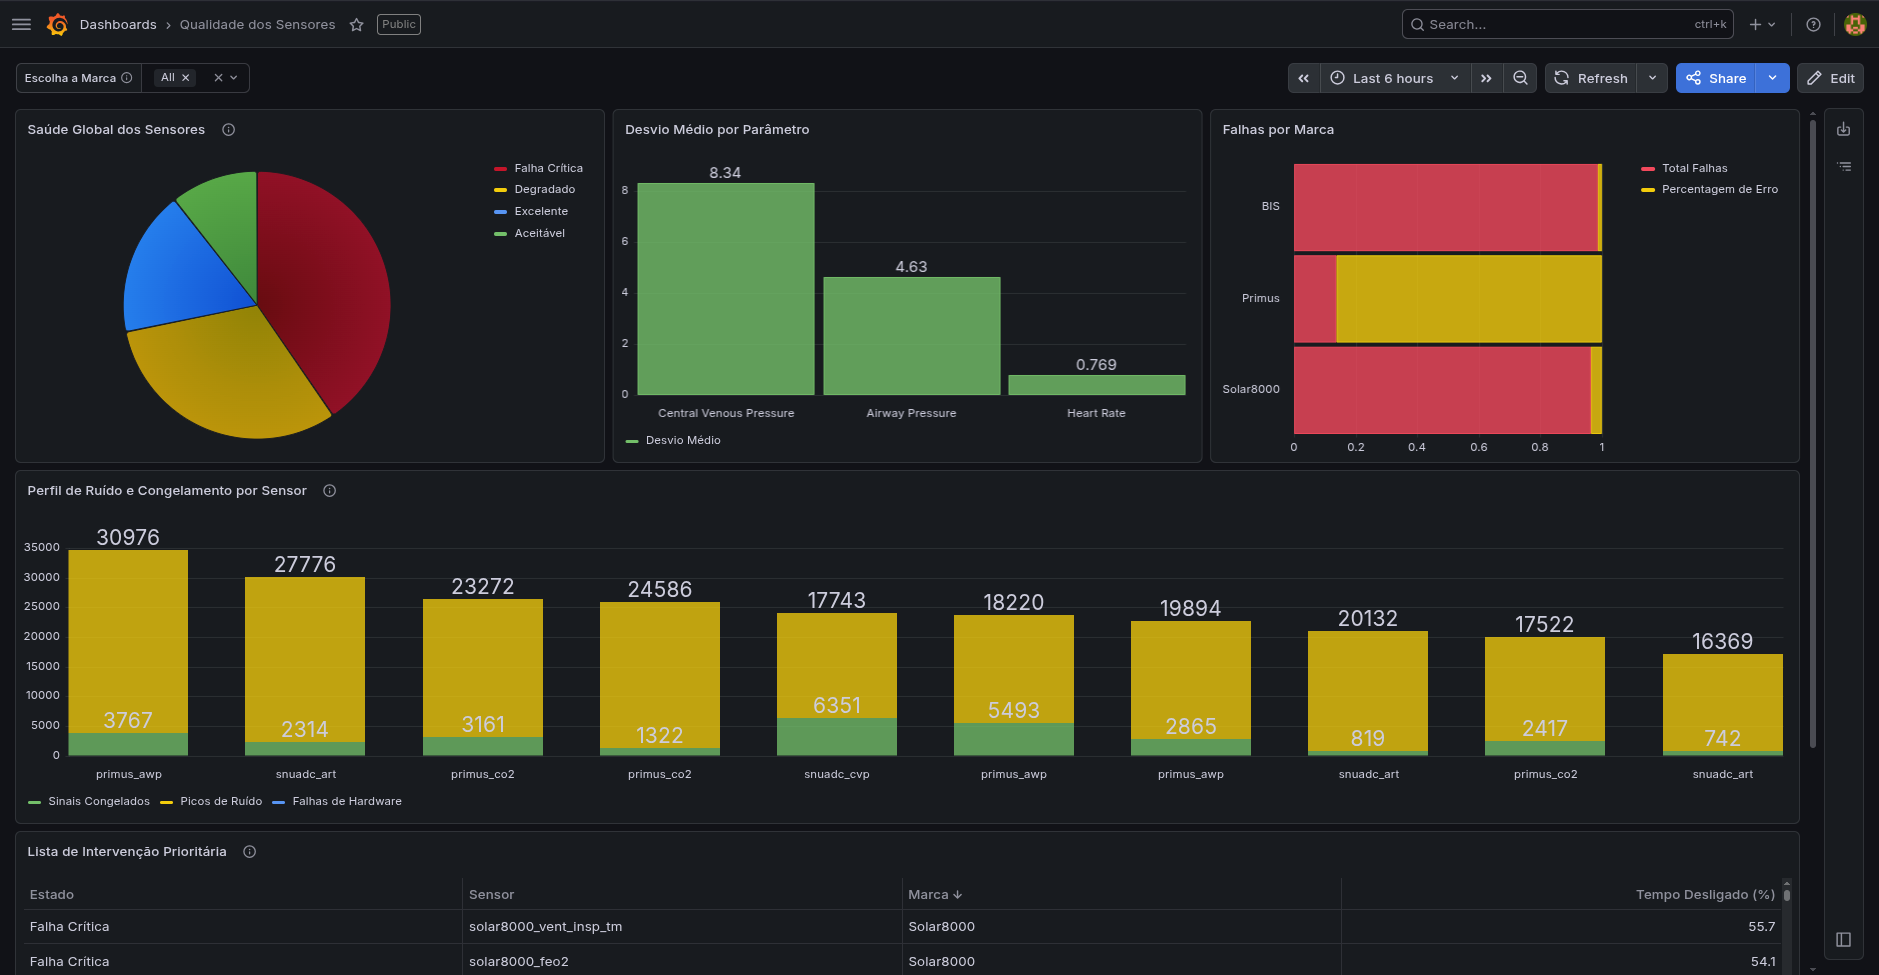
\includegraphics[width=0.7\linewidth]{imagens/qualidade_sensores_hugo}
	\caption{Dashboard Grafana de Saúde e Qualidade dos Sensores}
	\label{fig:qualidadesensoreshugo}
\end{figure}
\subsection{Pré. vs. Pós Operação} \label{subsec:pre_vs_pos_operacao}
O \textit{Dashboard} clínico pré e pós operatório permite medir o impacto e o cansaço causados pela cirurgia. Com base nos dados de todos os pacientes, o ecrã usa um gráfico \textit{Lollipop} para ajudar a equipa médica a ver rapidamente o que mudou em dezenas de análises ao sangue. Esta imagem mostra de forma clara o que desceu (linhas para a esquerda a rosa, ex: AMMO) e o que subiu ou se manteve (linhas para a direita a azul, ex: CCR ou PO2) logo a seguir à operação.

Além disso, a plataforma separa os resultados por género, usando gráficos de barras para mostrar as diferenças entre homens e mulheres. Este detalhe revela problemas que ficam escondidos quando olhamos apenas para a média geral. Por exemplo, mostra que a queda do valor de AMMO é muito mais grave nos homens.

Com a ajuda de filtros por especialidade médica e por indicador clínico, o painel transforma dados difíceis em informação clara e útil. Isto ajuda os médicos a planear melhor a recuperação de cada paciente.
\begin{figure}[h]
	\centering
	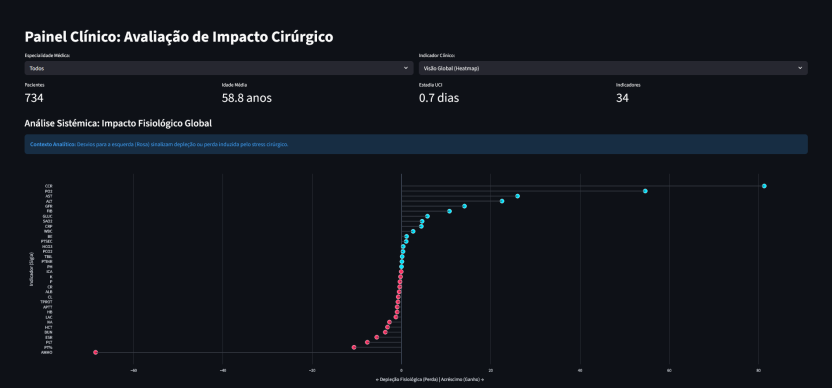
\includegraphics[width=0.7\linewidth]{imagens/pre_pos_operacao_duarte_1}
	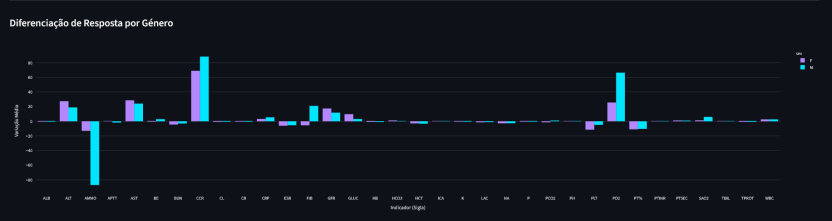
\includegraphics[width=0.7\linewidth]{imagens/pre_pos_operacao_duarte_2}
	\caption{Dashboard Streamlit Pré e Pós Operatório}
	\label{fig:preposoperacaoduarte}
\end{figure}

\subsection{Volatilidade dos Sinais Vitais} \label{subsec:volatilidade_sinais_vitais}
O dashboard desenvolvido tem como objetivo apoiar a interpretação dos sinais vitais recolhidos durante o procedimento cirúrgico, permitindo comparar o sinal bruto com o sinal suavizado e observar o efeito do processamento aplicado. A interface foi organizada em torno de filtros de cirurgia e sensor, o que possibilita ao utilizador selecionar rapidamente o contexto clínico pretendido e analisar a respetiva evolução temporal. Para melhorar a leitura dos resultados, o dashboard inclui ainda informação descritiva sobre cada sensor, como o parâmetro medido, a unidade de medida e a marca do equipamento, tornando a análise mais intuitiva e menos dependente de identificadores técnicos.

A página principal do relatório apresenta, lado a lado, o sinal antes e depois da suavização, facilitando a comparação entre a variabilidade original e a tendência subjacente após tratamento dos dados. Esta abordagem permite evidenciar a utilidade da suavização na redução de ruído e na interpretação clínica dos sinais. Além disso, a estrutura do dashboard foi pensada para ser interativo e orientada ao utilizador final, permitindo explorar os dados por cirurgia e por sensor sem necessidade de recorrer a consultas à base de dados. Desta forma, o dashboard transforma dados operacionais em informação visual mais clara, apoiando a análise exploratória e a comunicação dos resultados.

\begin{figure}[h]
	\centering
	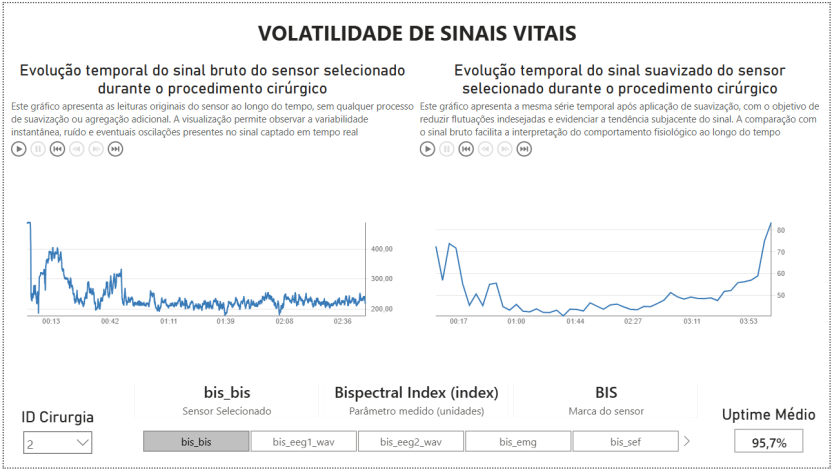
\includegraphics[width=0.7\linewidth]{imagens/volatilidade_nuno}
	\caption{Dashboard PowerBI de Volatilidade dos Sinais Vitais}
	\label{fig:volatilidadenuno}
\end{figure}

\subsection{Predições para Cuidados Intensivos}
O workflow de inferência do ICU Days Predictor foi implementado como uma pipeline do Flyte composto por quatro tarefas. Dado um ID relativo a um caso de paciente, a tarefa \textit{fetch\_case\_features} reconstrói o mesmo vetor de características utilizado durante o treino. Consultando a camada Silver, esta junta os dados demográficos do paciente (idade, sexo, IMC, score ASA) com o contexto cirúrgico (departamento, tipo de operação, abordagem, tipo de anestesia) e transforma os resultados laboratoriais pré-operatórios (hemoglobina, plaquetas, leucócitos, glicose, creatinina, albumina) numa única linha plana (flat row).

As tarefas \textit{find\_best\_regression\_model} e \textit{find\_best\_classification\_model} consultam o servidor do MLflow, classificando todas as execuções registadas na experiência \textit{ICU\_Days\_Regression} pelo menor RMSE, e na experiência \textit{ICU\_Days\_Classification} pelo maior AUC-ROC, devolvendo o URI do registo de modelos do vencedor.

Por último, a tarefa \textit{run\_predictions} carrega ambos os modelos a partir do MLflow Model Registry, aplica-os à linha de características e devolve um resultado estruturado em JSON contendo o número previsto de dias no UCI (regressão), o veredicto binário de admissão no UCI (classificação) e o valor real para comparação. Este design garante que a seleção do modelo seja sempre orientada por dados e reflita automaticamente qualquer reajuste futuro, sem a necessidade de atualizações manuais no pipeline de inferência.

\begin{figure}
	\centering
	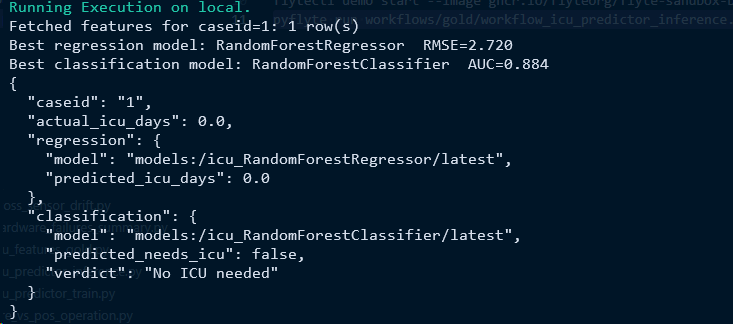
\includegraphics[width=0.7\linewidth]{imagens/predicoes_diogo}
	\caption{Output da Consola da Predição}
	\label{fig:predicoesdiogo}
\end{figure}
